% =====================================================================
%  Rapport de projet — Sélection de variables par AG vs BPSO
%  Structure conforme au cours « Méthodologie de recherche scientifique »
%  (A. Hadri, FSAO) : éléments préliminaires -> introduction générale ->
%  Ch.1 état de l'art -> Ch.2 matériels et méthodologie ->
%  Ch.3 résultats et discussion -> conclusion générale -> références -> annexes.
%
%  Overleaf : Menu > Compiler = pdfLaTeX (biber est lancé automatiquement).
%  Fichiers à téléverser à côté de ce .tex :
%    - references.bib
%    - resultats_auto.tex       (généré par la cellule 12 du notebook Colab)
%    - figures/convergence.png, figures/boxplot_precision.png
%  Tant que resultats_auto.tex est absent, les résultats apparaissent EN BLEU
%  comme emplacements réservés ; les zones EN ROUGE restent à compléter à la main.
% =====================================================================
\documentclass[11pt,a4paper]{report}

\usepackage[utf8]{inputenc}
\usepackage[T1]{fontenc}
\usepackage[french]{babel}
\usepackage{lmodern}
\usepackage{csquotes}
\usepackage[margin=2.5cm]{geometry}
\usepackage{amsmath,amssymb}
\usepackage{graphicx}
\usepackage{booktabs}
\usepackage{array}
\usepackage{xcolor}
\usepackage{caption}
\usepackage{algorithm}
\usepackage{algpseudocode}
\usepackage{float}
\usepackage[hidelinks]{hyperref}
\usepackage[backend=biber,style=ieee]{biblatex}   % style IEEE : informatique
\addbibresource{references.bib}

\newcommand{\todo}[1]{\textcolor{red}{\textbf{[À FAIRE : #1]}}}

% ---- Résultats : générés par le notebook (resultats_auto.tex) --------
\newcommand{\attente}[1]{\textcolor{blue}{\textbf{[Généré par le notebook : #1]}}}
\IfFileExists{resultats_auto.tex}{% Fichier généré automatiquement par le notebook le 24/10/2026 15:19
\newcommand{\NbRep}{%
10%
}

\newcommand{\TabAcc}{%
\begin{table}[H]
\centering
\caption{Précision sur le test en \% (moyenne $\pm$ écart-type sur $R = 10$ répétitions). Meilleure moyenne en gras.}
\label{tab:acc}
\begin{tabular}{@{}lcccc@{}}
\toprule
Jeu de données & Toutes & Filtre & AG & BPSO \\
\midrule
Breast Cancer & $\mathbf{96{,}3 \pm 1{,}4}$ & $96{,}0 \pm 1{,}6$ & $96{,}0 \pm 1{,}8$ & $96{,}0 \pm 1{,}3$ \\
Sonar & $80{,}0 \pm 4{,}6$ & $77{,}6 \pm 5{,}4$ & $\mathbf{81{,}3 \pm 6{,}4}$ & $79{,}4 \pm 5{,}3$ \\
Ionosphere & $83{,}3 \pm 2{,}1$ & $86{,}8 \pm 5{,}0$ & $\mathbf{88{,}0 \pm 3{,}6}$ & $87{,}0 \pm 2{,}6$ \\
\bottomrule
\end{tabular}
\end{table}%
}

\newcommand{\TabNvar}{%
\begin{table}[H]
\centering
\caption{Nombre de variables sélectionnées $|S|$ (moyenne $\pm$ écart-type). Plus petite moyenne en gras (hors Toutes).}
\label{tab:nvar}
\begin{tabular}{@{}lcccc@{}}
\toprule
Jeu de données & Toutes & Filtre & AG & BPSO \\
\midrule
Breast Cancer & $30$ & $22{,}0 \pm 0{,}0$ & $\mathbf{13{,}3 \pm 3{,}2}$ & $14{,}3 \pm 1{,}9$ \\
Sonar & $60$ & $29{,}4 \pm 11{,}0$ & $\mathbf{25{,}9 \pm 3{,}8}$ & $28{,}5 \pm 4{,}0$ \\
Ionosphere & $34$ & $\mathbf{6{,}8 \pm 6{,}8}$ & $7{,}8 \pm 1{,}2$ & $9{,}5 \pm 2{,}1$ \\
\bottomrule
\end{tabular}
\end{table}%
}

\newcommand{\TabTemps}{%
\begin{table}[H]
\centering
\caption{Temps moyen de sélection par exécution (secondes) et rapport au temps du filtre.}
\label{tab:temps}
\begin{tabular}{@{}lccccc@{}}
\toprule
Jeu de données & Filtre & AG & BPSO & AG / Filtre & BPSO / Filtre \\
\midrule
Breast Cancer & $0{,}18$ & $10{,}33$ & $13{,}98$ & $\times 57$ & $\times 78$ \\
Sonar & $0{,}16$ & $7{,}09$ & $9{,}18$ & $\times 44$ & $\times 58$ \\
Ionosphere & $0{,}17$ & $9{,}66$ & $12{,}29$ & $\times 56$ & $\times 72$ \\
\bottomrule
\end{tabular}
\end{table}%
}

\newcommand{\TabWilcoxon}{%
\begin{table}[H]
\centering
\caption{Test de Wilcoxon apparié, bilatéral (valeurs $p$ ; en gras si $p < 0{,}05$).}
\label{tab:wilcoxon}
\small
\begin{tabular}{@{}lcccccc@{}}
\toprule
 & \multicolumn{2}{c}{AG vs BPSO} & AG vs Filtre & BPSO vs Filtre & AG vs Toutes & BPSO vs Toutes \\
\cmidrule(lr){2-3}\cmidrule(lr){4-4}\cmidrule(lr){5-5}\cmidrule(lr){6-6}\cmidrule(lr){7-7}
Jeu de données & précision & $|S|$ & précision & précision & précision & précision \\
\midrule
Breast Cancer & $0{,}863$ & $0{,}467$ & $1{,}000$ & $1{,}000$ & $0{,}266$ & $0{,}477$ \\
Sonar & $0{,}416$ & $0{,}160$ & $0{,}258$ & $0{,}242$ & $0{,}523$ & $0{,}438$ \\
Ionosphere & $0{,}391$ & $\mathbf{0{,}008}$ & $0{,}586$ & $1{,}000$ & $\mathbf{0{,}004}$ & $\mathbf{0{,}004}$ \\
\bottomrule
\end{tabular}
\end{table}%
}

\newcommand{\FigConvergence}{%
\begin{figure}[H]
\centering
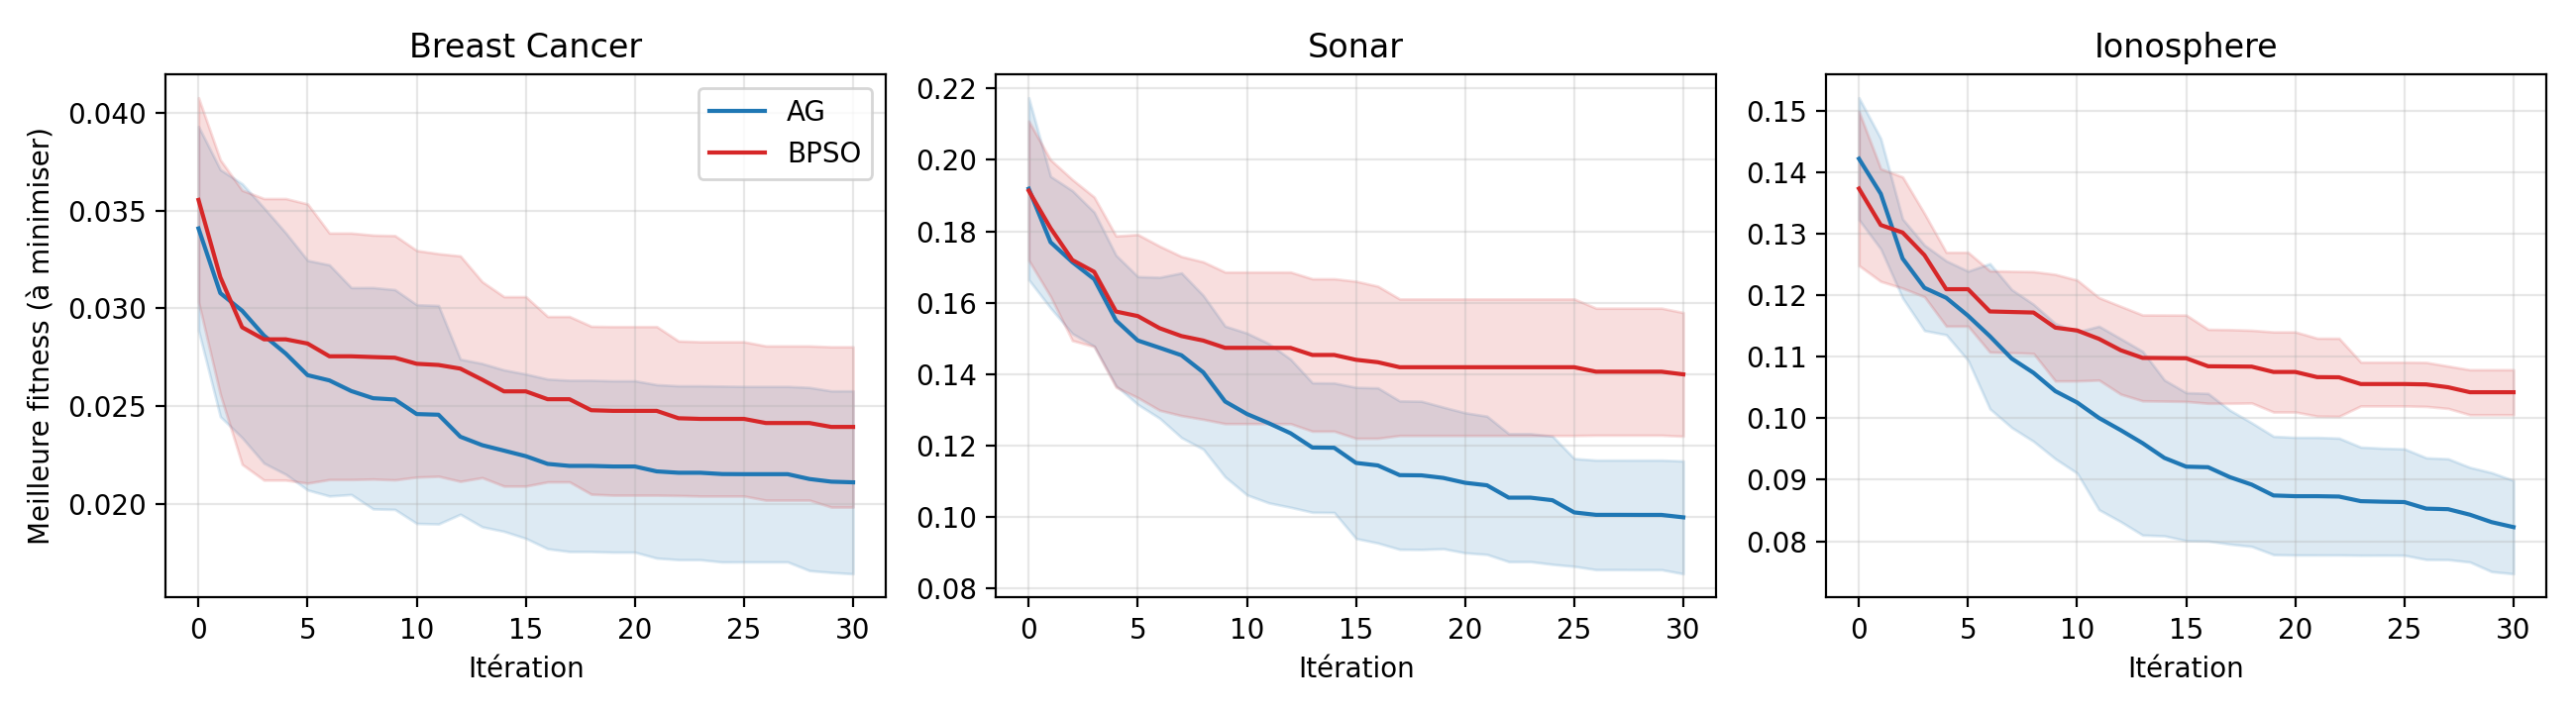
\includegraphics[width=\linewidth]{figures/convergence.png}
\caption{Convergence : meilleure fitness moyenne par itération ($\pm$ écart-type, 10 répétitions).}
\label{fig:convergence}
\end{figure}%
}

\newcommand{\FigBoxplot}{%
\begin{figure}[H]
\centering
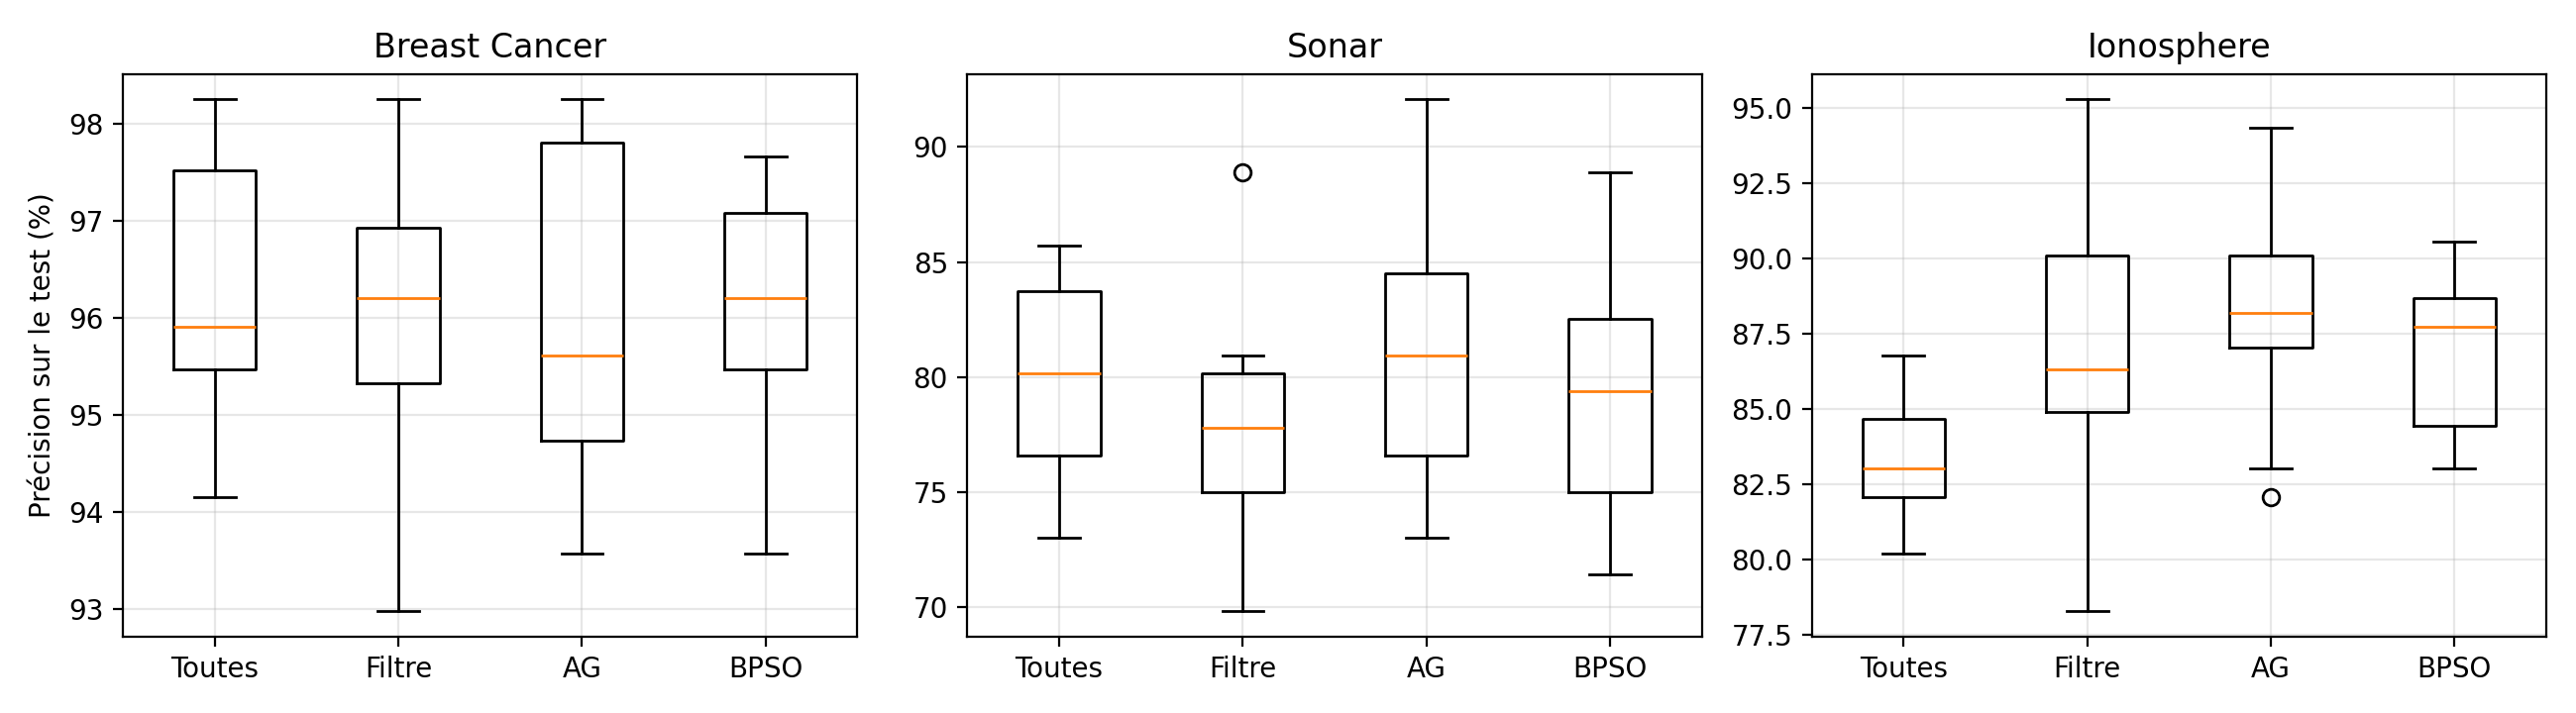
\includegraphics[width=\linewidth]{figures/boxplot_precision.png}
\caption{Distribution de la précision sur le test sur les 10 répétitions.}
\label{fig:boxplot}
\end{figure}%
}

\newcommand{\ResPrecision}{%
Sur Breast Cancer, la meilleure précision moyenne est obtenue par la référence Toutes (96{,}3~\%). Par rapport à l'utilisation de toutes les variables (96{,}3~\%), l'écart est de $-0{,}4$~point pour l'AG, $-0{,}3$~point pour le BPSO et $-0{,}4$~point pour le filtre.
Sur Sonar, la meilleure précision moyenne est obtenue par l'AG (81{,}3~\%). Par rapport à l'utilisation de toutes les variables (80{,}0~\%), l'écart est de $+1{,}3$~point pour l'AG, $-0{,}6$~point pour le BPSO et $-2{,}4$~points pour le filtre.
Sur Ionosphere, la meilleure précision moyenne est obtenue par l'AG (88{,}0~\%). Par rapport à l'utilisation de toutes les variables (83{,}3~\%), l'écart est de $+4{,}7$~points pour l'AG, $+3{,}7$~points pour le BPSO et $+3{,}5$~points pour le filtre.
Les écarts-types de la précision varient de 1{,}3 à 6{,}4~points selon la méthode et le jeu de données (tableau~\ref{tab:acc}, figure~\ref{fig:boxplot}).%
}

\newcommand{\ResVariables}{%
Sur Breast Cancer ($N = 30$), l'AG retient en moyenne 13{,}3 variables (44~\% de $N$), le BPSO 14{,}3 (48~\%) et le filtre 22{,}0 (73~\%).
Sur Sonar ($N = 60$), l'AG retient en moyenne 25{,}9 variables (43~\% de $N$), le BPSO 28{,}5 (48~\%) et le filtre 29{,}4 (49~\%).
Sur Ionosphere ($N = 34$), l'AG retient en moyenne 7{,}8 variables (23~\% de $N$), le BPSO 9{,}5 (28~\%) et le filtre 6{,}8 (20~\%).
L'écart-type moyen de $|S|$ entre répétitions est de 2{,}7 pour l'AG, 2{,}7 pour le BPSO et 5{,}9 pour le filtre (tableau~\ref{tab:nvar}).%
}

\newcommand{\ResTemps}{%
Le filtre sélectionne les variables en 0{,}16 à 0{,}18~s selon le jeu de données. La sélection par AG est 44 à 57 fois plus lente, et celle par BPSO 58 à 78 fois plus lente (tableau~\ref{tab:temps}).
À budget égal, le BPSO est plus lent que l'AG sur les trois jeux de données.
Le nombre d'évaluations étant identique, cet écart provient surtout du nombre de sous-ensembles distincts réellement évalués (la mémoïsation évite de réentraîner un masque déjà vu) et de la taille des sous-ensembles évalués.%
}

\newcommand{\ResSignif}{%
Sur Breast Cancer, la différence de précision entre AG et BPSO n'est pas significative ($p = 0{,}863$), et celle du nombre de variables n'est pas significative ($p = 0{,}467$). Par rapport au filtre, la différence de précision de l'AG n'est pas significative ($p = 1{,}000$) ; celle du BPSO n'est pas significative ($p = 1{,}000$).
Sur Sonar, la différence de précision entre AG et BPSO n'est pas significative ($p = 0{,}416$), et celle du nombre de variables n'est pas significative ($p = 0{,}160$). Par rapport au filtre, la différence de précision de l'AG n'est pas significative ($p = 0{,}258$) ; celle du BPSO n'est pas significative ($p = 0{,}242$).
Sur Ionosphere, la différence de précision entre AG et BPSO n'est pas significative ($p = 0{,}391$), et celle du nombre de variables est significative ($p = 0{,}008$). Par rapport au filtre, la différence de précision de l'AG n'est pas significative ($p = 0{,}586$) ; celle du BPSO n'est pas significative ($p = 1{,}000$).
Avec $R = 10$ répétitions, la plus petite valeur $p$ atteignable par le test de Wilcoxon bilatéral exact est d'environ $0{,}002$ (tableau~\ref{tab:wilcoxon}).%
}

\newcommand{\ResConvergence}{%
Sur Breast Cancer, l'AG atteint la meilleure fitness moyenne finale (AG : 0{,}0211 ; BPSO : 0{,}0239). L'AG réalise 95~\% de son amélioration totale à l'itération 21, le BPSO à l'itération 22.
Sur Sonar, l'AG atteint la meilleure fitness moyenne finale (AG : 0{,}0999 ; BPSO : 0{,}1399). L'AG réalise 95~\% de son amélioration totale à l'itération 25, le BPSO à l'itération 17.
Sur Ionosphere, l'AG atteint la meilleure fitness moyenne finale (AG : 0{,}0823 ; BPSO : 0{,}1042). L'AG réalise 95~\% de son amélioration totale à l'itération 27, le BPSO à l'itération 23.
La courbe moyenne de l'AG décroît encore au cours des cinq dernières itérations sur Breast Cancer, Sonar et Ionosphere, ce qui suggère qu'un budget plus élevé pourrait encore l'améliorer.
La courbe moyenne du BPSO décroît encore au cours des cinq dernières itérations sur Breast Cancer, Sonar et Ionosphere, ce qui suggère qu'un budget plus élevé pourrait encore l'améliorer.
(Figure~\ref{fig:convergence}.)%
}

\newcommand{\DiscHypotheses}{%
\textbf{H1 est confirmée} sur les trois jeux de données. Critère : sur un jeu de données, H1 est vérifiée si la précision de l'AG et du BPSO n'est pas significativement inférieure à celle de la référence Toutes et si chacun retient au plus la moitié des variables (tableaux~\ref{tab:acc}, \ref{tab:nvar} et \ref{tab:wilcoxon}).

\textbf{H2 est confirmée}. L'écart de précision entre la meilleure métaheuristique et le filtre vaut $+0{,}1$~point sur Breast Cancer, $+3{,}7$~points sur Sonar, $+1{,}2$~point sur Ionosphere ; il est le plus grand sur Sonar, qui est bien le jeu de plus grande dimension ($N = 60$).

\textbf{H3 est confirmée}. Le plus petit rapport de temps observé entre une métaheuristique et le filtre est de 44 (tableau~\ref{tab:temps}) ; le seuil d'un ordre de grandeur correspond à un rapport de 10.

\textbf{H4 est confirmée au sens faible} : le BPSO n'est significativement moins précis que l'AG sur aucun jeu de données (sa précision moyenne est supérieure ou égale sur 1 des 3 jeux), mais aucune différence n'est significative.%
}

\newcommand{\DiscLitterature}{%
Babaoğlu et al.~\cite{babaoglu2010} et Rafdi et al.~\cite{rafdi2021} rapportent un avantage du BPSO sur l'AG, chacun sur un seul jeu de données. Nos résultats nuancent cette tendance : à budget égal et sur trois jeux de données, aucune différence de précision entre AG et BPSO n'est statistiquement significative. L'avantage rapporté dans ces études, obtenu sur un seul jeu de données, ne se généralise donc pas ici.%
}

\newcommand{\DiscEcart}{%
Sur l'ensemble des répétitions, pour l'AG, la précision estimée en validation croisée sur l'apprentissage dépasse la précision mesurée sur le test de 5{,}1~points en moyenne ; pour le BPSO, la précision estimée en validation croisée sur l'apprentissage dépasse la précision mesurée sur le test de 3{,}9~points en moyenne. Cet écart positif montre que la fitness optimisée est une estimation optimiste : à force d'évaluer des centaines de sous-ensembles sur les mêmes plis, la recherche finit par exploiter des particularités de l'ensemble d'apprentissage. C'est précisément pour mesurer ce phénomène que la précision est rapportée sur un ensemble de test jamais utilisé pendant la sélection \cite{ambroise2002,kohavi1997}.%
}

\newcommand{\ReponseQuestion}{%
Dans nos conditions expérimentales, l'AG n'améliore significativement la précision du filtre sur aucun jeu de données, alors que sa sélection est 44 à 57 fois plus lente : du point de vue de la précision, son coût de calcul n'est pas justifié.%
}

\newcommand{\ResumeChiffres}{%
Sur Sonar (60 variables), l'AG atteint 81{,}3~\% de précision avec 25{,}9 variables en moyenne, le BPSO 79{,}4~\% avec 28{,}5 variables et le filtre 77{,}6~\% avec 29{,}4 variables, contre 80{,}0~\% avec toutes les variables ; la sélection par AG est 44 fois plus lente que le filtre. Dans nos conditions expérimentales, l'AG n'améliore significativement la précision du filtre sur aucun jeu de données, alors que sa sélection est 44 à 57 fois plus lente : du point de vue de la précision, son coût de calcul n'est pas justifié.%
}

\newcommand{\AbstractNumbers}{%
On Sonar (60 features), the GA reaches 81.3\% accuracy with 25.9 features on average, BPSO 79.4\% with 28.5 features and the filter 77.6\% with 29.4 features, versus 80.0\% with all features; GA selection is 44 times slower than the filter. Under our experimental conditions, the GA does not significantly improve on the filter's accuracy on any dataset, while being 44 to 57 times slower: in terms of accuracy, its computational cost is not justified.%
}

\newcommand{\ConclusionChapitre}{%
Les résultats établissent les points suivants : H1 est confirmée, H2 est confirmée, H3 est confirmée et H4 est confirmée au sens faible. Dans nos conditions expérimentales, l'AG n'améliore significativement la précision du filtre sur aucun jeu de données, alors que sa sélection est 44 à 57 fois plus lente : du point de vue de la précision, son coût de calcul n'est pas justifié.%
}

\newcommand{\Environnement}{%
Les expériences ont été réalisées sous Python 3.13.16 avec NumPy 2.1.3 et scikit-learn 1.6.1 (Google Colab, processeur x86\_64, 2 cœurs). La durée totale des expériences est d'environ 11~min.%
}

}{%
  \newcommand{\NbRep}{10}
  \newcommand{\TabAcc}{\attente{tableau de précision}}
  \newcommand{\TabNvar}{\attente{tableau du nombre de variables}}
  \newcommand{\TabTemps}{\attente{tableau des temps}}
  \newcommand{\TabWilcoxon}{\attente{tableau des tests de Wilcoxon}}
  \newcommand{\FigConvergence}{\attente{figure de convergence}}
  \newcommand{\FigBoxplot}{\attente{figure des précisions}}
  \newcommand{\ResPrecision}{\attente{description de la précision}}
  \newcommand{\ResVariables}{\attente{description du nombre de variables}}
  \newcommand{\ResTemps}{\attente{description des temps}}
  \newcommand{\ResSignif}{\attente{description des tests}}
  \newcommand{\ResConvergence}{\attente{description de la convergence}}
  \newcommand{\DiscHypotheses}{\attente{vérification des hypothèses H1 à H4}}
  \newcommand{\DiscLitterature}{\attente{comparaison avec la littérature}}
  \newcommand{\DiscEcart}{\attente{écart entre validation croisée et test}}
  \newcommand{\ReponseQuestion}{\attente{réponse à la question de recherche}}
  \newcommand{\ResumeChiffres}{\attente{résultats chiffrés du résumé}}
  \newcommand{\AbstractNumbers}{\attente{numerical results of the abstract}}
  \newcommand{\ConclusionChapitre}{\attente{conclusion du chapitre 3}}
  \newcommand{\Environnement}{\attente{environnement logiciel}}
}

\floatname{algorithm}{Algorithme}
\renewcommand{\algorithmicrequire}{\textbf{Entrée :}}
\renewcommand{\algorithmicensure}{\textbf{Sortie :}}

% =====================================================================
\begin{document}

% =====================================================================
%                     ÉLÉMENTS PRÉLIMINAIRES
% =====================================================================
\begin{titlepage}
\centering
{\large Université Ibn Zohr | Faculté des Sciences Appliquées de Ouarzazate\par}
{\large Master Intelligence Artificielle et Applications (IAA)\par}
\vspace{0.5cm}
{Module : {Optimisation numerique}\par}
\vspace{3cm}
{\LARGE\bfseries Sélection de variables pour la classification par Algorithme Génétique :\\[0.3cm]
comparaison avec PSO binaire et une référence simple\par}
\vspace{2.5cm}
{\large Réalisé par :\par}
\vspace{0.2cm}
{\large \textbf{Hamza Oukhacha} \quad et \quad \textbf{EL-JANDOUZ HASSANE}\par}
\vspace{0.4cm}
{\large Encadré par : {Pr. Aissam Hadri}\par}
\vfill
{\large Année universitaire 2026--2027\par}
\end{titlepage}

\pagenumbering{roman}

% ------------------------------------------------------------------
\chapter*{Remerciements}
\addcontentsline{toc}{chapter}{Remerciements}
Nous tenons à exprimer nos sincères remerciements à notre professeur, Issam Hadri, pour son encadrement, ses explications claires et ses conseils sur la rédaction d'un rapport dans le respect des règles de la recherche scientifique. Son soutien nous a permis de surmonter les difficultés techniques et de mener ce travail à bien, de la meilleure manière possible.

% ------------------------------------------------------------------
% Structure du résumé (cours, diapo 38) :
% contexte -> justification -> objectif -> méthode -> résultats chiffrés -> conclusion.
% À FINALISER EN DERNIER : il ne doit contenir aucun résultat absent du rapport.
\chapter*{Résumé}
\addcontentsline{toc}{chapter}{Résumé}
La sélection de variables vise à retenir, parmi les variables d'un jeu de données, un
sous-ensemble réduit qui préserve ou améliore la performance d'un classifieur.
Ce problème combinatoire est souvent traité par des métaheuristiques coûteuses, dont l'apport
réel face à des méthodes simples est rarement mesuré à budget égal. Ce
travail compare un algorithme génétique (AG) et une optimisation par essaim particulaire binaire
(BPSO) à deux références simples : l'utilisation de toutes les variables et un filtre univarié
(\emph{objectif}). Les deux métaheuristiques disposent du même budget de 620 évaluations ; toutes
les méthodes sont évaluées avec un classifieur k-NN sur trois jeux de données de référence, selon
un protocole de 10 répétitions où la sélection n'utilise jamais l'ensemble de test, et les
différences sont testées par le test de Wilcoxon.
\ResumeChiffres

\medskip
\noindent\textbf{Mots-clés :} sélection de variables ; approche wrapper ; algorithme génétique ;
optimisation par essaim particulaire binaire ; classification ; k plus proches voisins.

% ------------------------------------------------------------------
\chapter*{Abstract}
\addcontentsline{toc}{chapter}{Abstract}
Feature selection aims to retain a small subset of the original variables that preserves or
improves classifier performance. This combinatorial problem is often addressed with costly
metaheuristics, whose actual benefit over simple methods is rarely measured under an equal
budget. This work compares a genetic algorithm (GA) and binary particle swarm optimization (BPSO)
with two simple baselines: using all features and a univariate filter (ANOVA F). Both
metaheuristics receive the same budget of 620 fitness evaluations. All methods are evaluated with
a k-NN classifier on three benchmark datasets, using 10 repetitions in which the test set is never
used for selection; differences are assessed with the Wilcoxon signed-rank test.
\AbstractNumbers

\medskip
\noindent\textbf{Keywords:} feature selection; wrapper approach; genetic algorithm; binary
particle swarm optimization; classification; k-nearest neighbors.

% ------------------------------------------------------------------
\tableofcontents
\listoffigures
\listoftables

\chapter*{Liste des abréviations et symboles}
\addcontentsline{toc}{chapter}{Liste des abréviations et symboles}
\begin{tabular}{@{}ll@{}}
AG    & Algorithme génétique \\
PSO   & Optimisation par essaim particulaire (\emph{Particle Swarm Optimization}) \\
BPSO  & PSO binaire (\emph{Binary PSO}) \\
k-NN  & $k$ plus proches voisins (\emph{k-Nearest Neighbors}) \\
CV    & Validation croisée (\emph{Cross-Validation}) \\
ANOVA & Analyse de la variance \\
$N$   & Nombre total de variables d'un jeu de données \\
$n$   & Nombre d'exemples d'un jeu de données \\
$S$, $|S|$ & Sous-ensemble de variables sélectionnées, et sa taille \\
$f$   & Fonction objectif (fitness), à minimiser \\
$\alpha$ & Poids de l'erreur de classification dans $f$ \\
$P$, $T$ & Taille de la population (ou de l'essaim) et nombre d'itérations \\
$R$   & Nombre de répétitions indépendantes de l'expérience \\
\end{tabular}

\cleardoublepage
\pagenumbering{arabic}

% =====================================================================
%                     INTRODUCTION GÉNÉRALE
% Plan du cours (diapo 59) : contexte -> problématique -> état des
% connaissances -> lacune -> objectifs -> démarche -> organisation.
% =====================================================================
\chapter*{Introduction générale}
\addcontentsline{toc}{chapter}{Introduction générale}
\markboth{Introduction générale}{Introduction générale}

\section*{Contexte}
En apprentissage automatique, les jeux de données contiennent de plus en plus de variables
(\emph{features}). Dans certains domaines, comme l'analyse de l'expression des gènes ou la
classification de textes, une seule observation peut être décrite par des dizaines de milliers de
variables \cite{guyon2003}. Or toutes ces variables ne sont pas utiles : beaucoup d'entre elles
sont non pertinentes ou redondantes \cite{xue2016}. Leur présence expose au \emph{fléau de la
dimension} et pose trois problèmes \cite{guyon2003} :
\begin{enumerate}
  \item elle ralentit l'entraînement et l'utilisation des modèles de classification ;
  \item elle augmente le risque de surapprentissage (\emph{overfitting}) : le modèle apprend le
        bruit des données au lieu des régularités utiles ;
  \item elle rend le modèle plus difficile à interpréter.
\end{enumerate}

Pour y remédier, on utilise la \emph{sélection de variables}, qui consiste à retenir uniquement un
sous-ensemble de variables pertinentes, sans les transformer. Parmi les approches proposées, les
algorithmes d'optimisation bio-inspirés, comme les algorithmes génétiques (AG)
\cite{holland1975,yang1998} et l'optimisation par essaim particulaire binaire (BPSO)
\cite{kennedy1997}, sont largement étudiés \cite{xue2016,agrawal2021,dokeroglu2022}. Ces méthodes
évaluent chaque sous-ensemble candidat en entraînant le classifieur lui-même à chaque étape de la
recherche : c'est l'approche dite \emph{wrapper} \cite{kohavi1997}.

\section*{Problématique}
Trouver le meilleur sous-ensemble de variables est un problème combinatoire classé NP-difficile
\cite{xue2016,dokeroglu2022}. Pour $N$ variables, il existe $2^N$ sous-ensembles possibles
\cite{kohavi1997} : pour le jeu Sonar ($N = 60$), cela représente environ
$1{,}15 \times 10^{18}$ combinaisons. Même à raison de 10~ms par évaluation, une recherche
exhaustive dépasserait 300~millions d'années.

Deux familles de solutions s'opposent alors. Les méthodes \emph{filtres} classent chaque variable
selon un critère statistique ; elles sont rapides, mais évaluent les variables une à une, sans
tenir compte de leurs interactions \cite{guyon2003,xue2016}. Les méthodes \emph{wrapper} prennent
en compte ces interactions et obtiennent en général une meilleure précision, au prix d'un coût de
calcul élevé \cite{xue2016,dokeroglu2022}. Les métaheuristiques comme l'AG et le BPSO
appartiennent à cette seconde famille : elles exigent elles-mêmes beaucoup de ressources
\cite{xue2016,ludwig2025}, et, d'après le théorème \emph{No Free Lunch}, aucune n'est garantie
d'être la meilleure sur tous les problèmes \cite{dokeroglu2022}. Les comparaisons directes entre
AG et BPSO rapportent d'ailleurs un avantage du BPSO, mais chacune sur un seul jeu de données et
avec un classifieur différent \cite{babaoglu2010,rafdi2021}, ce qui ne permet pas de généraliser. Enfin, de nombreux travaux souffrent d'un
biais de sélection, lorsque les données de test interviennent dans le choix des variables
\cite{xue2016,ambroise2002} ; une comparaison fiable doit donc l'éviter.

\section*{Question de recherche et hypothèses}
Cela nous amène à la question de recherche de ce projet :

\begin{quote}
\textbf{Dans le cadre d'un problème de classification, l'utilisation d'un algorithme génétique pour
sélectionner les variables justifie-t-elle son coût de calcul par rapport au PSO binaire et à une
méthode filtre simple ?}
\end{quote}

\noindent Plus précisément, l'étude cherche à répondre aux questions suivantes :
\begin{itemize}
  \item[\textbf{Q1}] À budget d'évaluations égal, l'AG obtient-il une meilleure précision de
        classification, moins de variables ou un temps de calcul plus court que le BPSO ?
  \item[\textbf{Q2}] L'AG et le BPSO apportent-ils une amélioration statistiquement significative
        par rapport à un filtre simple (test ANOVA F), nettement plus rapide à exécuter ?
\end{itemize}

\medskip
\noindent Hypothèses, formulées \emph{avant} les expériences :
\begin{itemize}
  \item[\textbf{H1}] (Q2) AG et BPSO atteignent une précision au moins comparable à celle de la
        référence utilisant toutes les variables, avec nettement moins de variables.
  \item[\textbf{H2}] (Q2) L'avantage des métaheuristiques sur le filtre est plus marqué sur le jeu
        de données de plus grande dimension (Sonar, $N = 60$), où les interactions entre variables
        sont plus nombreuses.
  \item[\textbf{H3}] (question principale) Le temps de sélection des métaheuristiques dépasse celui
        du filtre d'au moins un ordre de grandeur.
  \item[\textbf{H4}] (Q1) Conformément aux comparaisons publiées \cite{babaoglu2010,rafdi2021},
        le BPSO obtient une précision au moins égale à celle de l'AG ; nous testons si cet avantage
        se confirme à budget égal et sur plusieurs jeux de données.
\end{itemize}

\section*{Objectifs}
\begin{enumerate}
  \item Implémenter un AG et un BPSO pour la sélection de variables, avec la même fonction
        objectif et le même budget d'évaluations.
  \item Les comparer à deux références simples selon trois critères mesurables : précision sur
        l'ensemble de test, nombre de variables retenues et temps de calcul.
  \item Tester la significativité statistique des différences observées.
\end{enumerate}

\section*{Démarche adoptée}
La démarche est \emph{quantitative et expérimentale} : la question porte sur des performances
mesurables, et les hypothèses sont testées par des expériences répétées suivies d'un test
statistique. Ce travail ne propose pas un nouvel algorithme ; sa contribution est une comparaison
\emph{contrôlée} : budget identique, référence filtre réglée de façon équitable, protocole sans
fuite de l'ensemble de test, et code entièrement reproductible.

\section*{Organisation du rapport}
Le chapitre~\ref{chap:etat-art} présente la méthodologie de recherche documentaire suivie et
l'état de l'art. Le chapitre~\ref{chap:methodo} décrit les jeux de données, la formulation du
problème, les méthodes comparées et le protocole expérimental. Le chapitre~\ref{chap:resultats}
présente puis discute les résultats. Une conclusion générale résume les apports et propose des
perspectives.

% =====================================================================
\chapter{État de l'art}
\label{chap:etat-art}
% =====================================================================
\section{Introduction du chapitre}
Ce chapitre a pour objectif de situer le projet dans la littérature. Il décrit d'abord la
démarche de recherche documentaire suivie, puis présente les familles de méthodes de sélection
de variables, les deux métaheuristiques étudiées et une synthèse critique des travaux existants,
qui conduit au positionnement du projet.

% ---------------------------------------------------------------------
\section{Méthodologie de la recherche documentaire}
\label{sec:recherche-doc}

\subsection{De la question de recherche aux mots-clés}
La question de recherche a été décomposée en quatre concepts, puis chaque concept a été traduit
en anglais avec ses synonymes et acronymes (tableau~\ref{tab:mots-cles}).

\begin{table}[H]
\centering
\caption{Concepts de la question de recherche et mots-clés associés.}
\label{tab:mots-cles}
\begin{tabular}{@{}>{\raggedright}p{3.4cm}p{10.6cm}@{}}
\toprule
Concept & Mots-clés en anglais (synonymes, acronymes) \\
\midrule
Sélection de variables & \textit{feature selection}, \textit{feature subset selection},
                         \textit{variable selection}, \textit{wrapper} \\
Algorithme génétique   & \textit{genetic algorithm}, \textit{evolutionary algorithm},
                         \textit{evolutionary computation} \\
PSO binaire            & \textit{particle swarm optimization}, PSO, BPSO,
                         \textit{binary PSO}, \textit{transfer function} \\
Classification         & \textit{classification}, \textit{classifier}, k-NN \\
\bottomrule
\end{tabular}
\end{table}

\subsection{Requête et bases interrogées}
Les concepts ont été combinés avec les opérateurs booléens \texttt{OR} (synonymes d'un même
concept) et \texttt{AND} (concepts différents) :

\begin{center}
\begin{minipage}{0.92\linewidth}
\small\ttfamily
("feature selection" OR "feature subset selection" OR "variable selection")\\
AND ("genetic algorithm*" OR "particle swarm" OR BPSO)\\
AND classif*
\end{minipage}
\end{center}

La recherche a été menée sur Google Scholar, IEEE Xplore et ScienceDirect, avec deux filtres : période 2015--2026 pour les travaux récents (sans filtre de
date pour les articles fondateurs), et documents de type article de revue ou de conférence en
informatique. Les résultats ont été triés par nombre de citations pour repérer les travaux
fondateurs et par date pour repérer les travaux récents.

% Faites réellement la recherche et remplissez ce tableau avec VOS chiffres.
\begin{table}[H]
\centering
\caption{Résultats de la recherche documentaire.}
\label{tab:recherche-doc}
\begin{tabular}{@{}lccc@{}}
\toprule
Base & Résultats bruts & Après filtres & Retenus après lecture \\
\midrule
Google Scholar & {17\,600} & {17\,400} & {20+} \\
ScienceDirect  & {1\,032} & {79} & {40} \\
IEEE Xplore    & {} & {} & {} \\
\bottomrule
\end{tabular}
\end{table}

\subsection{Critères de sélection et organisation}
Un document a été retenu s'il (i) traite de la sélection de variables pour la classification,
(ii) décrit sa méthode de façon reproductible, et (iii) provient d'une source identifiable : revue
indexée, conférence avec comité de lecture ou ouvrage de référence. Les sources ont été combinées
selon leur rôle : articles fondateurs, revues de synthèse et travaux récents. Les références ont
été gérées avec Zotero et exportées au format BibTeX ; pour chaque article lu, une fiche de lecture
(objectif, méthode, résultats, limites) a été remplie (annexe~\ref{ann:lecture}).

% ---------------------------------------------------------------------
\section{Familles de méthodes de sélection de variables}
On distingue classiquement trois familles de méthodes \cite{guyon2003}.
\begin{itemize}
  \item Les méthodes \textbf{filtres} attribuent un score à chaque variable à l'aide d'un critère
        statistique (corrélation, test ANOVA F, information mutuelle), indépendamment de tout
        classifieur.
  \item Les méthodes \textbf{wrapper} évaluent chaque \emph{sous-ensemble} candidat par la
        performance du classifieur lui-même \cite{kohavi1997}. Une méthode wrapper associe une
        \emph{stratégie de recherche} dans l'espace des sous-ensembles à une \emph{fonction
        d'évaluation}.
  \item Les méthodes \textbf{embarquées} réalisent la sélection pendant l'apprentissage du modèle,
        par exemple par régularisation $L_1$ (Lasso) ou par l'importance des variables dans les
        arbres de décision.
\end{itemize}
Le tableau~\ref{tab:familles} compare ces familles selon quatre critères explicites.

\begin{table}[H]
\centering
\caption{Comparaison des familles de méthodes de sélection de variables.}
\label{tab:familles}
\begin{tabular}{@{}lccc@{}}
\toprule
Critère & Filtre & Wrapper & Embarquée \\
\midrule
Coût de calcul                           & faible & élevé  & moyen \\
Prise en compte des interactions          & non (univarié) & oui & partielle \\
Dépendance au classifieur                 & non    & oui    & oui (modèle imposé) \\
Risque de sur-apprentissage de la sélection & faible & élevé & moyen \\
\bottomrule
\end{tabular}
\end{table}

\noindent Ce projet compare deux \emph{stratégies de recherche} wrapper (AG et BPSO) avec la même
fonction d'évaluation, et les confronte à un filtre.

% ---------------------------------------------------------------------
\section{Algorithmes génétiques pour la sélection de variables}
Les algorithmes génétiques, introduits par Holland \cite{holland1975} et popularisés par
Goldberg \cite{goldberg1989}, imitent l'évolution naturelle : une population de solutions évolue
par sélection des meilleurs individus, croisement et mutation. Le codage binaire, où chaque gène
indique la présence ou l'absence d'une variable, rend l'AG naturellement adapté à la sélection de
variables. Yang et Honavar \cite{yang1998} ont été parmi les premiers à l'appliquer à ce
problème, avec une fonction objectif combinant la précision d'un réseau de neurones et le coût
des variables retenues.

% ---------------------------------------------------------------------
\section{PSO et sa version binaire}
L'optimisation par essaim particulaire (PSO) a été proposée par Kennedy et Eberhart
\cite{kennedy1995}, en s'inspirant du déplacement collectif des vols d'oiseaux. Chaque particule
se déplace en combinant sa vitesse précédente, l'attraction vers sa meilleure position passée et
l'attraction vers la meilleure position de l'essaim. La version d'origine opère dans un espace
continu. Les mêmes auteurs ont proposé une version binaire (BPSO) \cite{kennedy1997} : la vitesse
reste réelle, mais elle est transformée par une fonction sigmoïde en \emph{probabilité} que le bit
correspondant vaille 1. Mirjalili et Lewis \cite{mirjalili2013} ont montré que le choix de cette
fonction de transfert (en forme de S ou de V) influence fortement les performances du BPSO.

% ---------------------------------------------------------------------
\section{Synthèse critique et positionnement}
Les revues de synthèse \cite{xue2016,agrawal2021,dokeroglu2022} montrent que les
métaheuristiques, et en particulier l'AG et le PSO, occupent une place centrale dans la littérature
sur la sélection de variables, avec un nombre de variantes en forte croissance. Xue et al.
\cite{xue2016} soulignent aussi que le coût de calcul des approches wrapper et la rigueur du
protocole d'évaluation restent des points délicats. Le tableau~\ref{tab:etat-art} résume les
travaux sur lesquels s'appuie ce projet.

% Conseil : vérifiez chaque « limite » en lisant l'article, et corrigez-la si besoin.
\begin{table}[H]
\centering
\caption{Synthèse de travaux représentatifs.}
\label{tab:etat-art}
\small
\begin{tabular}{@{}>{\raggedright}p{3cm}>{\raggedright}p{4.3cm}>{\raggedright}p{2.7cm}p{4.2cm}@{}}
\toprule
Référence & Méthode & Évaluation & Limite relevée \\
\midrule
Kohavi et John \cite{kohavi1997} & Wrapper, recherche heuristique (hill-climbing, best-first)
  & Arbre ID3, Naïve Bayes & Coût de calcul élevé \\
Yang et Honavar \cite{yang1998} & AG à codage binaire, fitness précision + coût
  & Réseau de neurones & Résultats liés au classifieur choisi \\
Kennedy et Eberhart \cite{kennedy1997} & Introduction du BPSO (fonction sigmoïde)
  & Fonctions de test & Pas d'application à la sélection de variables \\
Mirjalili et Lewis \cite{mirjalili2013} & BPSO, fonctions de transfert en S et en V
  & Fonctions de test & Pas d'application à la sélection de variables \\
\midrule
Babaoğlu et al.\ \cite{babaoglu2010} & BPSO vs AG en mode wrapper, 23 variables
  & SVM, CV $k$ plis ; 1 jeu médical & Un seul jeu de données \\
Rafdi et al.\ \cite{rafdi2021} & PSO vs AG pour l'analyse de sentiments
  & Naïve Bayes ; 1 jeu Twitter & Un seul jeu ; paramètres non précisés dans le résumé \\
Ludwig \cite{ludwig2025} & BPSO guidé, initialisé par des filtres ; comparé à BPSO, AG, ANOVA
  & k-NN ; 12 jeux génomiques ($> 35\,000$ variables) & Coût de calcul élevé (signalé par l'auteur) \\
\bottomrule
\end{tabular}
\end{table}

\noindent Les comparaisons directes entre AG et BPSO rapportent un avantage du BPSO : Babaoğlu
et al.\ \cite{babaoglu2010} l'observent pour le diagnostic de la maladie coronarienne avec un
SVM, et Rafdi et al.\ \cite{rafdi2021} pour l'analyse de sentiments avec un classifieur bayésien
naïf. Ces deux études portent toutefois chacune sur un seul jeu de données. Sur des données
génomiques de très grande dimension, Ludwig \cite{ludwig2025} compare un BPSO amélioré à
plusieurs méthodes, dont l'AG, le BPSO standard et un filtre ANOVA, et observe des résultats de
précision partagés entre les variantes de PSO, avec un temps d'exécution élevé.

\noindent La lacune visée par ce projet n'est pas algorithmique mais méthodologique. Les
comparaisons AG/BPSO disponibles reposent sur un seul jeu de données \cite{babaoglu2010,rafdi2021}
ou sur des données d'une dimension très éloignée des jeux usuels \cite{ludwig2025}. Ce projet
compare l'AG et le BPSO sur plusieurs jeux de dimension moyenne, à budget égal, sans fuite de
l'ensemble de test, et face à un filtre simple, afin de mesurer ce que la complexité des
métaheuristiques apporte réellement.

\section{Conclusion du chapitre}
L'état de l'art établit trois points : la sélection de variables est un problème combinatoire
pour lequel les métaheuristiques wrapper sont très utilisées ; l'AG et le BPSO reposent sur un
codage binaire directement adapté au problème ; leur coût et la rigueur de leur évaluation restent
discutés. Le chapitre suivant décrit le dispositif expérimental conçu pour répondre à la question
de recherche.

% =====================================================================
\chapter{Matériels et méthodologie}
\label{chap:methodo}
% =====================================================================
\section{Introduction du chapitre}
Ce chapitre décrit précisément comment les résultats ont été obtenus, afin qu'un autre chercheur
puisse les reproduire : jeux de données, formulation du problème, méthodes comparées, protocole
expérimental, critères d'évaluation et environnement logiciel.

% ---------------------------------------------------------------------
\section{Jeux de données}
Trois jeux de données de référence, à deux classes, sont utilisés (tableau~\ref{tab:datasets}).
Ils sont publics et couramment employés dans la littérature sur la sélection de variables, ce
qui rend l'expérience reproductible.

\begin{table}[H]
\centering
\caption{Jeux de données utilisés (source : UCI Machine Learning Repository \cite{uci}).}
\label{tab:datasets}
\begin{tabular}{@{}lrrl@{}}
\toprule
Jeu de données & $n$ (exemples) & $N$ (variables) & Tâche \\
\midrule
Breast Cancer Wisconsin & 569 & 30 & tumeur bénigne / maligne \\
Sonar                   & 208 & 60 & signal sonar : mine / roche \\
Ionosphere              & 351 & 34 & signal radar : bon / mauvais \\
\bottomrule
\end{tabular}
\end{table}

% ---------------------------------------------------------------------
\section{Formulation du problème}
\label{sec:formulation}
Une solution est un vecteur binaire
\[
\mathbf{x} = (x_1, \dots, x_N) \in \{0,1\}^N,
\]
où $x_j = 1$ signifie que la variable $j$ est sélectionnée. On note
$S = \{\, j : x_j = 1 \,\}$ et $|S|$ le nombre de variables retenues. La fonction objectif, à
\textbf{minimiser}, est :
\begin{equation}
f(\mathbf{x}) = \alpha \,\bigl(1 - \mathrm{Acc}_{\mathrm{CV}}(S)\bigr)
              + (1-\alpha)\,\frac{|S|}{N},
\label{eq:fitness}
\end{equation}
où $\mathrm{Acc}_{\mathrm{CV}}(S)$ est la précision moyenne d'un k-NN ($k=5$) en validation
croisée à 5 plis \textbf{sur l'ensemble d'apprentissage uniquement}, et $\alpha = 0{,}99$.
Si $|S| = 0$, on pose $f(\mathbf{x}) = 1$.

Cette formulation, qui combine l'erreur de classification et la proportion de variables
retenues, est courante dans la littérature ; Ludwig \cite{ludwig2025} l'utilise également avec un
classifieur k-NN. Le paramètre $\alpha$ fixe la priorité entre les deux objectifs. Avec $\alpha = 0{,}99$, la
précision domine : le terme $|S|/N$ sert surtout à départager deux sous-ensembles de précision
voisine, en favorisant le plus petit. Avec $\alpha = 1$, seule la précision compterait ; avec
$\alpha = 0{,}5$, réduire le nombre de variables pèserait autant que réduire l'erreur.

% ---------------------------------------------------------------------
\section{Méthodes comparées}
\subsection{Références simples}
\begin{itemize}
  \item \textbf{Toutes} : toutes les variables sont utilisées, sans sélection.
  \item \textbf{Filtre} : les variables sont classées par le score du test ANOVA F, puis les $k$
        meilleures sont conservées ; $k$ est choisi par validation croisée sur l'apprentissage
        parmi 10\,\%, 20\,\%, 30\,\%, 50\,\% et 75\,\% de $N$.
\end{itemize}

\subsection{Algorithme génétique (AG)}
Chaque individu est un vecteur binaire de longueur $N$, initialisé en tirant chaque bit à 1 avec
une probabilité de 0,5. À chaque génération, les parents sont choisis par \emph{tournoi} de
taille 3 : trois individus sont tirés au hasard et le meilleur est retenu. Deux parents
produisent deux enfants par \emph{croisement uniforme} (probabilité $p_c = 0{,}9$) : chaque gène
est hérité de l'un ou l'autre parent avec une probabilité de 1/2. Chaque gène des enfants est
ensuite inversé avec une probabilité $p_m = 1/N$, soit en moyenne une mutation par individu.
Enfin, l'\emph{élitisme} copie le meilleur individu tel quel dans la génération suivante, ce qui
garantit que la meilleure fitness ne se dégrade jamais (algorithme~\ref{alg:ga}).

\begin{algorithm}[H]
\caption{Algorithme génétique pour la sélection de variables}
\label{alg:ga}
\begin{algorithmic}[1]
\Require taille de population $P$, générations $T$, probabilités $p_c$, $p_m$
\Ensure meilleur masque $\mathbf{x}^\star$
\State Initialiser $P$ vecteurs binaires aléatoires ; évaluer $f$ ; mémoriser le meilleur $\mathbf{x}^\star$
\For{$t = 1$ \textbf{à} $T$}
  \State Nouvelle population $\gets \{\mathbf{x}^\star\}$ \Comment{élitisme}
  \While{la nouvelle population compte moins de $P$ individus}
    \State Choisir deux parents par tournoi de taille 3
    \State Avec probabilité $p_c$, appliquer le croisement uniforme
    \State Inverser chaque bit des enfants avec probabilité $p_m$ ; ajouter les enfants
  \EndWhile
  \State Évaluer $f$ ; mettre à jour $\mathbf{x}^\star$
\EndFor
\State \Return $\mathbf{x}^\star$
\end{algorithmic}
\end{algorithm}

\subsection{PSO binaire (BPSO)}
Pour chaque particule $i$ et chaque dimension $d$, la vitesse est mise à jour par :
\begin{equation}
v_{id}^{t+1} = w\, v_{id}^{t}
             + c_1 r_1 \bigl(p_{id} - x_{id}^{t}\bigr)
             + c_2 r_2 \bigl(g_{d} - x_{id}^{t}\bigr),
\label{eq:vitesse}
\end{equation}
puis la nouvelle position est tirée à l'aide de la fonction de transfert sigmoïde :
\begin{equation}
S(v) = \frac{1}{1 + e^{-v}}, \qquad
x_{id}^{t+1} =
\begin{cases}
1 & \text{si } r < S\bigl(v_{id}^{t+1}\bigr),\\
0 & \text{sinon},
\end{cases}
\label{eq:sigmoide}
\end{equation}
avec $r_1, r_2, r \sim \mathcal{U}(0,1)$, $\mathbf{p}_{i}$ la meilleure position passée de la
particule $i$, $\mathbf{g}$ la meilleure position de l'essaim, et $v \in [-v_{\max}, v_{\max}]$.

Dans l'équation~\eqref{eq:vitesse}, le terme $w\,v_{id}^{t}$ (\emph{inertie}) conserve une partie
du mouvement précédent ; le terme \emph{cognitif} $c_1 r_1 (p_{id} - x_{id}^{t})$ attire la
particule vers sa propre meilleure solution ; le terme \emph{social} $c_2 r_2 (g_{d} - x_{id}^{t})$
l'attire vers la meilleure solution de l'essaim. Une vitesse fortement positive rend la valeur 1
très probable, une vitesse fortement négative rend la valeur 0 très probable. L'inertie $w$
décroît linéairement de 0,9 à 0,4 : l'essaim explore largement au début, puis se concentre
autour des meilleures solutions. Le bornage $v_{\max} = 6$ limite l'amplitude des vitesses
(algorithme~\ref{alg:bpso}).

\begin{algorithm}[H]
\caption{PSO binaire pour la sélection de variables}
\label{alg:bpso}
\begin{algorithmic}[1]
\Require particules $P$, itérations $T$, $w_{\max}$, $w_{\min}$, $c_1$, $c_2$, $v_{\max}$
\Ensure meilleur masque $\mathbf{g}$
\State Initialiser positions binaires et vitesses ; évaluer $f$ ; initialiser $\mathbf{p}_i$ et $\mathbf{g}$
\For{$t = 1$ \textbf{à} $T$}
  \State $w \gets w_{\max} - (w_{\max} - w_{\min})\,(t-1)/(T-1)$
  \For{chaque particule $i$}
    \State Mettre à jour la vitesse (éq.~\ref{eq:vitesse}) et la borner dans $[-v_{\max}, v_{\max}]$
    \State Tirer la nouvelle position (éq.~\ref{eq:sigmoide})
    \State Évaluer $f$ ; mettre à jour $\mathbf{p}_i$ si la solution est meilleure
  \EndFor
  \State Mettre à jour $\mathbf{g}$
\EndFor
\State \Return $\mathbf{g}$
\end{algorithmic}
\end{algorithm}

\subsection{Équité de la comparaison}
AG et BPSO disposent du \textbf{même budget} : $P = 20$ individus et $T = 30$ itérations, soit
$20 + 20 \times 30 = 620$ évaluations de $f$ par exécution (tableau~\ref{tab:params}). Au sein
d'une même répétition, ils utilisent les mêmes plis de validation croisée, donc exactement la même
fonction objectif. Un masque déjà évalué est mémorisé et n'est pas réentraîné, ce qui accélère le
calcul sans modifier le budget compté.

\begin{table}[H]
\centering
\caption{Paramètres des métaheuristiques.}
\label{tab:params}
\begin{tabular}{@{}lll@{}}
\toprule
Paramètre & AG & BPSO \\
\midrule
Taille de population & 20 & 20 \\
Itérations & 30 & 30 \\
Spécifiques & tournoi $= 3$, $p_c = 0{,}9$, $p_m = 1/N$ & $w$ : $0{,}9 \to 0{,}4$, $c_1 = c_2 = 2$, $v_{\max} = 6$ \\
\bottomrule
\end{tabular}
\end{table}

% ---------------------------------------------------------------------
\section{Protocole expérimental}
Pour chaque répétition $r = 0, \dots, R-1$ (avec $R = 10$) :
\begin{enumerate}
  \item découpage stratifié 70\,\% apprentissage / 30\,\% test (graine $r$) ;
  \item standardisation ajustée sur l'apprentissage seulement ;
  \item sélection des variables par chaque méthode, \textbf{sur l'apprentissage seulement} ;
  \item entraînement d'un k-NN ($k = 5$) sur les variables retenues et mesure sur le test.
\end{enumerate}
Les quatre méthodes partagent le même découpage à chaque répétition. La sélection n'utilise
jamais l'ensemble de test, afin d'éviter le biais de sélection décrit par Ambroise et McLachlan
\cite{ambroise2002}, qui rend les performances artificiellement optimistes.

% ---------------------------------------------------------------------
\section{Critères d'évaluation et analyse statistique}
Trois mesures sont relevées pour chaque méthode : la précision sur l'ensemble de test, le nombre
de variables sélectionnées $|S|$ et le temps de sélection en secondes. Elles sont résumées par la
moyenne et l'écart-type sur les $R$ répétitions.

Comme les méthodes partagent le même découpage, les mesures sont \emph{appariées}. Les différences
sont donc testées par le test des rangs signés de Wilcoxon, bilatéral, au seuil de 0,05
\cite{demsar2006}. Ce test non paramétrique ne suppose pas la normalité des différences, ce qui
convient à un petit nombre de répétitions.

% ---------------------------------------------------------------------
\section{Environnement logiciel et reproductibilité}
\Environnement
L'implémentation repose sur scikit-learn \cite{sklearn}. Toutes les graines aléatoires sont
fixées, et le code complet est fourni (annexe~\ref{ann:code}).

\section{Conclusion du chapitre}
Le dispositif décrit garantit trois conditions : une fonction objectif et un budget identiques
pour l'AG et le BPSO, une sélection réalisée sans accès à l'ensemble de test, et des mesures
appariées permettant un test statistique. Le chapitre suivant présente les résultats obtenus dans
ces conditions.

% =====================================================================
\chapter{Résultats et discussion}
\label{chap:resultats}
% =====================================================================
\section{Introduction du chapitre}
Ce chapitre présente les résultats dans l'ordre des objectifs annoncés (précision, nombre de
variables, temps de calcul, significativité), puis les interprète au regard des hypothèses et de
la littérature.

% Les paragraphes de résultats sont rédigés automatiquement par le notebook à partir des
% données (règle du cours : décrire les tendances avec un vocabulaire mesurable).
% Relisez-les : vous devez pouvoir justifier chaque phrase.

\section{Précision de classification}
\TabAcc
\ResPrecision

\FigBoxplot

\section{Nombre de variables sélectionnées}
\TabNvar
\ResVariables

\section{Temps de calcul}
\TabTemps
\ResTemps

\section{Significativité statistique}
\TabWilcoxon
\ResSignif

\section{Convergence des métaheuristiques}
\FigConvergence
\ResConvergence

% ---------------------------------------------------------------------
\section{Discussion}
\subsection{Vérification des hypothèses}
\DiscHypotheses

\subsection{Interprétation}
\paragraph{Filtre et interactions entre variables.}
Le filtre ANOVA évalue chaque variable isolément \cite{guyon2003}. Lorsqu'il obtient une
précision comparable à celle des métaheuristiques, cela indique que, sur ces jeux de données,
les variables utiles le sont déjà individuellement : la prise en compte des interactions, qui est
l'avantage théorique des approches wrapper \cite{kohavi1997,xue2016}, n'apporte alors qu'un gain
limité. À l'inverse, un avantage significatif d'une métaheuristique signale des variables utiles
seulement en combinaison.

\paragraph{Sur-apprentissage du critère de sélection.}
\DiscEcart

\paragraph{Nombre de variables et rôle de $\alpha$.}
Avec $\alpha = 0{,}99$, la fonction objectif~\eqref{eq:fitness} privilégie fortement la
précision : réduire le nombre de variables ne rapporte qu'un gain très faible. Les
métaheuristiques n'ont donc pas de raison forte de produire des sous-ensembles plus petits que
le filtre, dont la taille $k$ est choisie par validation croisée. Un poids $\alpha$ plus faible
conduirait à des sous-ensembles plus compacts, au prix d'une précision éventuellement moindre.

\paragraph{Variabilité des solutions.}
L'AG et le BPSO sont des algorithmes stochastiques : d'une graine à l'autre, ils peuvent produire
des sous-ensembles différents \cite{xue2016}. Les écarts-types de $|S|$ rapportés dans le
tableau~\ref{tab:nvar} mesurent cette instabilité, alors que le filtre, déterministe pour un
découpage donné, ne varie qu'avec les données d'apprentissage.

\subsection{Comparaison avec la littérature}
\DiscLitterature{} Ces comparaisons restent qualitatives : les études citées utilisent d'autres
jeux de données, d'autres classifieurs (SVM, Naïve Bayes) et ne précisent pas toujours le budget
d'évaluations, ce qui empêche de comparer directement les valeurs de précision. Ludwig
\cite{ludwig2025}, qui emploie comme ici un k-NN et un filtre ANOVA, observe également un coût de
calcul élevé des variantes de PSO ; nos mesures de temps (tableau~\ref{tab:temps}) vont dans ce
sens à plus petite échelle.

\subsection{Limites}
Ces conclusions restent limitées par plusieurs choix. Seules $R = \NbRep$ répétitions ont été
réalisées, ce qui réduit la puissance du test statistique. Un seul classifieur (k-NN) a été
utilisé : les sous-ensembles sélectionnés pourraient ne pas convenir à un autre modèle. Les
paramètres des métaheuristiques n'ont pas été optimisés, et un budget plus élevé aurait pu
modifier le classement. Enfin, trois jeux de données de dimension moyenne ne permettent pas de
généraliser à des données de grande dimension (plusieurs milliers de variables).

\section{Conclusion du chapitre}
\ConclusionChapitre

% =====================================================================
\chapter*{Conclusion générale et perspectives}
\addcontentsline{toc}{chapter}{Conclusion générale et perspectives}
\markboth{Conclusion générale}{Conclusion générale}
% Question directrice du cours : qu'avons-nous appris, démontré ou réalisé ?
Ce projet avait pour objectif de déterminer si deux métaheuristiques, l'AG et le BPSO, apportent
un gain mesurable par rapport à une méthode filtre simple pour la sélection de variables, à budget
égal et selon un protocole sans fuite de l'ensemble de test.

Pour y répondre, un AG et un BPSO ont été implémentés avec la même fonction objectif et le même
budget, puis comparés à l'utilisation de toutes les variables et à un filtre ANOVA, sur trois
jeux de données et dix répétitions appariées. \ReponseQuestion

Ce résultat rejoint une idée centrale de la méthodologie expérimentale : une méthode complexe
doit toujours être comparée à une référence simple, réglée avec le même soin, avant de conclure
à son intérêt.

La contribution de ce travail est méthodologique : un protocole de comparaison équitable et
entièrement reproductible, réutilisable pour évaluer d'autres méthodes de sélection.

Plusieurs prolongements découlent de ces résultats : tester des fonctions de transfert en V pour
le BPSO \cite{mirjalili2013}, évaluer les sous-ensembles avec d'autres classifieurs, étendre
l'étude à des jeux de données de plus grande dimension, et traiter la précision et le nombre de
variables comme deux objectifs distincts dans une approche multi-objectif.

% =====================================================================
\printbibliography[heading=bibintoc, title={Références}]

% =====================================================================
\appendix

\chapter{Code source et reproductibilité}
\label{ann:code}
\sloppy
Toutes les expériences sont reproductibles à partir du notebook
\texttt{projet\_selection\_variables.ipynb} (Google Colab), qui fixe toutes les graines
aléatoires et génère automatiquement les tableaux et figures du chapitre~\ref{chap:resultats}.
Le notebook est fourni avec ce rapport. Il produit également les fichiers de résultats bruts
(\texttt{resultats\_bruts.csv}), le résumé statistique (\texttt{resume.csv}) et les valeurs $p$
(\texttt{wilcoxon.csv}), ainsi que le fichier \texttt{resultats\_auto.tex} inséré dans le
chapitre~\ref{chap:resultats}.

\chapter{Fiches de lecture}
\label{ann:lecture}
% Fiches établies à partir des résumés et des sections lues. Complétez-les après lecture complète.
\begin{table}[H]
\centering
\caption{Fiches de lecture des principaux articles.}
\label{tab:fiches}
\small
\begin{tabular}{@{}>{\raggedright}p{2.6cm}>{\raggedright}p{2.8cm}>{\raggedright}p{2.8cm}>{\raggedright}p{2.8cm}p{2.8cm}@{}}
\toprule
Référence & Objectif & Méthode & Résultats & Limites \\
\midrule
Xue et al. \cite{xue2016} & Revue des approches évolutionnaires pour la sélection de variables
  & Synthèse par algorithme (AG, PSO, etc.) et par type d'évaluation (filtre, wrapper)
  & Approches largement utilisées pour leur capacité de recherche globale
  & Défis : coût de calcul, passage à l'échelle, stabilité, biais de sélection \\
Mirjalili et Lewis \cite{mirjalili2013} & Étudier la fonction de transfert du BPSO
  & Comparaison de fonctions en S et en V sur des fonctions de test
  & Les fonctions en V améliorent nettement le BPSO
  & Pas d'évaluation en sélection de variables \\
Dokeroglu et al. \cite{dokeroglu2022} & Revue des métaheuristiques récentes pour la sélection
  & Synthèse des travaux récents, classifieurs et réglages
  & Problème NP-difficile ; aucune métaheuristique universelle (No Free Lunch)
  & Réglage des paramètres et équilibre exploration/exploitation ouverts \\
Babaoğlu et al. \cite{babaoglu2010} & Comparer BPSO et AG pour le diagnostic coronarien
  & SVM, validation croisée $k$ plis, 23 variables
  & BPSO plus précis que l'AG et que toutes les variables
  & Un seul jeu de données \\
Rafdi et al. \cite{rafdi2021} & Améliorer un Naïve Bayes en analyse de sentiments
  & Sélection par PSO et par AG, validation croisée
  & Précision : 60,3\,\% sans sélection, 77,5\,\% (PSO), 70,7\,\% (AG)
  & Un seul jeu ; réglages non détaillés dans le résumé \\
Ludwig \cite{ludwig2025} & BPSO guidé, initialisé par des filtres
  & k-NN, 12 jeux génomiques, test de Mann--Whitney
  & Précision partagée avec le BPSO ; meilleur F1 sur plusieurs jeux
  & Coût de calcul élevé \\
\bottomrule
\end{tabular}
\end{table}


\end{document}